\documentclass[10pt,article]{article}
\usepackage{pdfpages}
\usepackage[letterpaper,margin=0.3in]{geometry}
\usepackage{graphicx}
\usepackage{booktabs}
\usepackage{url}
\usepackage{enumitem}
\usepackage{palatino}
\usepackage{tabularx}
\fontfamily{SansSerif}
\selectfont

\usepackage[UTF8]{ctex}
\usepackage[T1]{fontenc}
\usepackage
%[ansinew]
[utf8]
{inputenc}

\usepackage{color}
\definecolor{mygrey}{gray}{0.82}
\textheight=9.75in
\raggedbottom

\setlength{\tabcolsep}{0in}
\newcommand{\isep}{-2 pt}
\newcommand{\lsep}{-0.5cm}
\newcommand{\psep}{-0.6cm}
\renewcommand{\labelitemii}{$\circ$}

\pagestyle{empty}
%-----------------------------------------------------------
%Custom commands
\newcommand{\resitem}[1]{\item #1 \vspace{-2pt}}
\newcommand{\resheading}[1]{{\small \colorbox{mygrey} { \begin{minipage}{0.99\textwidth}\centering{\textbf{#1 \vphantom{p\^{E}}}}\end{minipage}}}}
\newcommand{\ressubheading}[3]{
	\begin{tabular*}{6.62in}{l @{\extracolsep{\fill}} r}
		\textsc{{\textbf{#1}}} & \rightline\textsc{\textit{[#2]}} \\
	\end{tabular*}\vspace{-8pt}}
%-----------------------------------------------------------

\begin{document}

	\begin{table}[h]
		\begin{minipage}{0\linewidth}
			\centering
			
\includegraphics[height =0.8in]{./whulogo.png}
		\end{minipage}
		\begin{minipage}{0.9\linewidth}
			%\centering
			\setlength{\tabcolsep}{70pt}
			\def\arraystretch{1.1}
			\begin{tabular}{ll}
				\textbf{\Large{易守拙}}  &  {手机：+86 13667280239} \\
				\textbf{计算机学院,计算机科学与技术} &  {邮箱：yishouzhuo@whu.edu.cn} \\
				\textbf{武汉大学}
			\end{tabular}
		\end{minipage}
		\begin{minipage}{0\linewidth}
			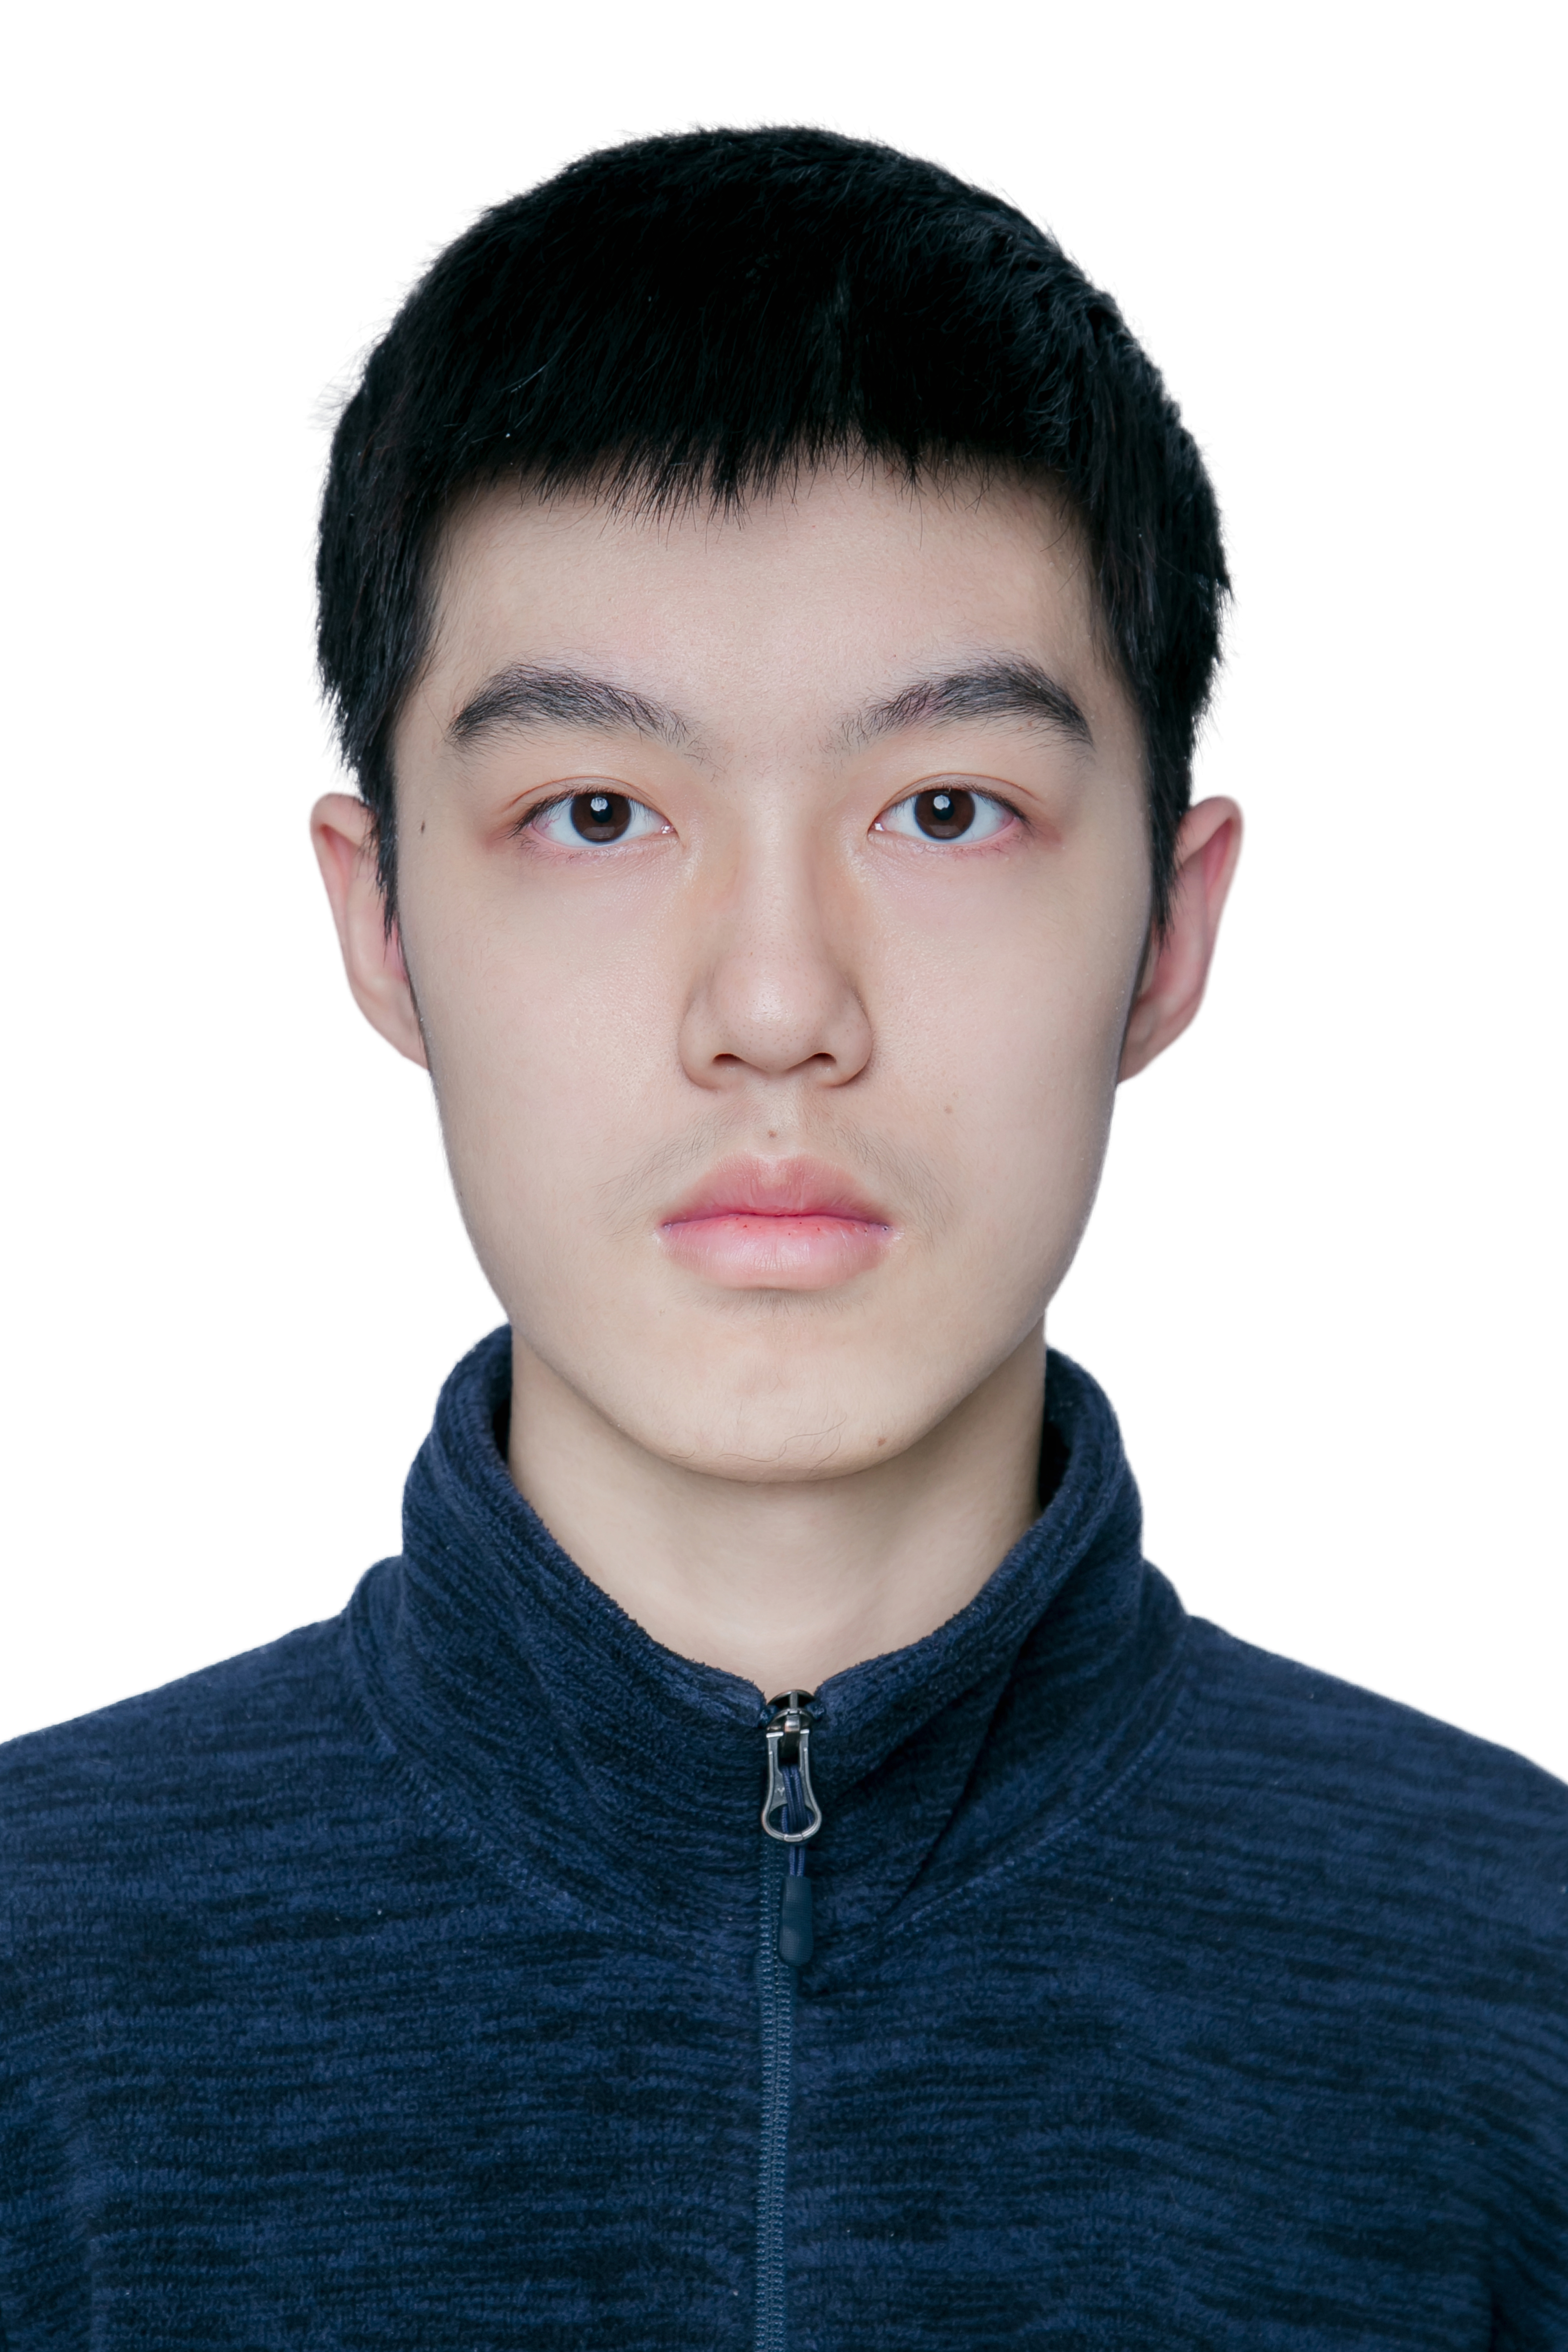
\includegraphics[height =1in]{photo.png}
		\end{minipage}\hfill
	\end{table}
	
	\noindent
	\resheading{\textbf{校内成绩}}\\[-0.5cm]
	\begin{itemize}
		\setlength\itemsep{-0.45em}
		\item 主修专业:计算机科学与技术(计算机弘毅班) \hfill {[2024 - 2028]}
		\\目前就读大二 
		\\绩点：3.84/4.00   
		\\均分: 92.55/100 (排名:4/30)
		\\四级成绩: 608
		\\修读的专业课和成绩:高级语言程序设计A(97),数据结构A(97),计算机系统基础(88),软件系统实践(96)
	%	\\排名：9/30
		\\[-0.6cm]
	\end{itemize}
	
	
	\noindent
	\resheading{\textbf{科研经历}}\\[-0.45cm]
	\begin{itemize}
		\setlength\itemsep{-0.2em}
		
		\item \textbf{武汉大学智能感知与机器学习研究组}\hfill {[2025.9-]} 
		\begin{itemize}[noitemsep,nolistsep]
			\item 指导老师：刘友发副研究员(武汉大学计算机学院)
			\item 研究内容:  基于大型视觉语言模型的无源迁移学习
		%	\item 研究成果:  学术论文在撰
		\end{itemize}
		
	\end{itemize}
	\noindent
	\resheading{\textbf{项目经历}}\\[-0.45cm]
	\begin{itemize}
		\setlength\itemsep{-0.2em}
		
		\item \textbf{基于Winsocket以及Qt5的局域网聊天室搭建}\hfill {[2024.11-2024.12]} 
		\begin{itemize}[noitemsep,nolistsep]
			\item 指导老师：刘峰(武汉大学计算机学院)
			\item 课程: 高级语言程序设计A大作业
			%	\item 研究成果:  学术论文在撰
		\end{itemize}
		
	\end{itemize}
	
	\noindent
	\resheading{\textbf{我的技能 
		%	\& 我的科研兴趣
		}}\\[-0.5cm]
	\begin{itemize}
		\item \textbf{编程语言}: C++ , Python\\[-0.7cm]
%	\item \textbf{掌握的的软件工具}: LTSpice，ADS，MATLAB，Tina90  \\[-0.7cm]
       \item \textbf{掌握的论文写作工具}：LaTeX, Word \\[-0.7cm]
	%	\item \textbf{我的科研兴趣}: 多模态大模型,具身智能,计算机视觉\\[-0.5cm]
	\end{itemize}
	
	
	\noindent
	\resheading{\textbf{获得的奖项}}\\[-0.2cm]
	% \textbf{Econometrics | Statistics | Mathematical Methods | Microeconomics | Macroeconomics}\hfill {[ISI-D]}\\[-0.1cm]\\
	\begin{itemize}[noitemsep,nolistsep]
		
		\item \textbf{2024-2025学年优秀学生奖学金}\hfill {[校级]}\\[-0.4cm] 
		
		\item \textbf{2024-2025第十六届蓝桥杯省赛 C/C++ 大学 A 组二等奖}\hfill {[省级]}\\[-0.4cm]
		
		\item \textbf{2024-2025学年优秀学生}\hfill {[校级]}\\[-0.4cm]
		
	\end{itemize}
	
	
	%\noindent
	%\resheading{\textbf{自我评价}}\\[-0.2cm]
	% \textbf{Econometrics | Statistics | Mathematical Methods | Microeconomics | Macroeconomics}\hfill {[ISI-D]}\\[-0.1cm]\\
	%\begin{itemize}[noitemsep,nolistsep]
	% \item{我在三年的学习过程中，团结同学，认真细致，勤于反思，不断进步。抗挫折能力较强，遇到问题能以良好的心态解决。}\\[-0.4cm]\\
	%\end{itemize}
		
		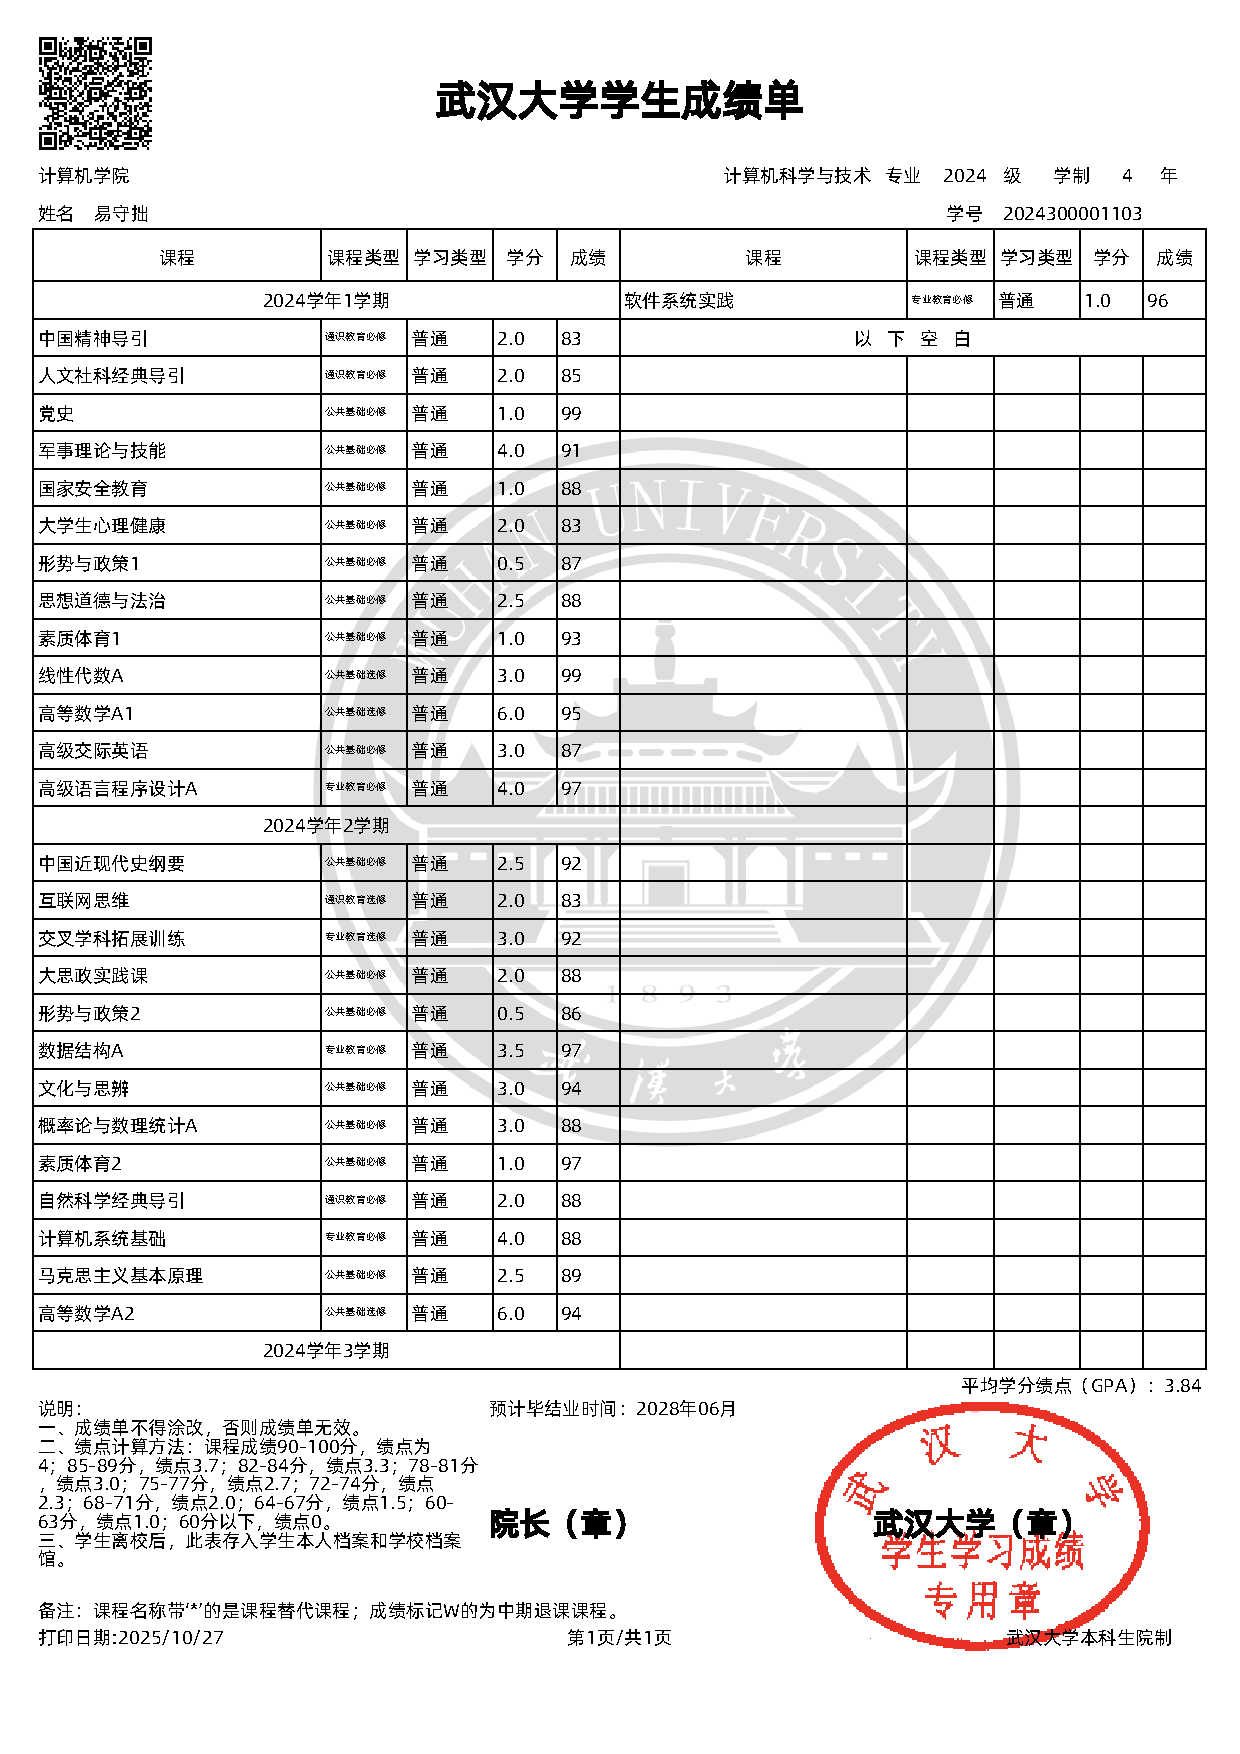
\includepdf[pages=1]{GPA大二上.pdf}
\end{document}